\section{Aufgabe 5}
Im folgenden wir $U$ immer als die vorrausgesetzte Gleichverteilung angesehen.
Da die Algorithmen effizient sein sollen, wird im folgenden die Methode der Transformierung der Gleichverteilung genutzt.

\subsection{a)}
Normierung:
\begin{align*}
  &\int_{x_{\symup{min}}}^{x_{\symup{max}}} A \symup{d}x = A(x_{\symup{max}}-x_{\symup{min}}) = 1 \\
  => \; &A=\frac{1}{x_{\symup{max}}-x_{\symup{min}}}
\end{align*}
Trasformation:
\begin{align*}
  U &= \int_{x_{\symup{min}}}^{x} \frac{1}{x_{\symup{max}}-x_{\symup{min}}} \symup{d}x'\\
  &= \left[ \frac{1}{x_{\symup{max}}-x_{\symup{min}}} \cdot x' \right]_{x_{\symup{min}}}^{x} \\
  &= \frac{x-x_{\symup{min}}}{x_{\symup{max}}-x_{\symup{min}}}
\end{align*}
Inverse bilden:
\begin{align*}
  x(U) = U \cdot (x_{\symup{max}}-x_{\symup{min}}) + x_{\symup{min}}
\end{align*}
In Abbildung \ref{5.a} ist die resultierende, normierte Verteilung mit den Parametern
\begin{align*}
  x_{\symup{min}} &= -100 \\
  x_{\symup{max}} &= 100
\end{align*}
zu sehen. Für das Histogramm wurden 1 Millionen Zufallswerte genommen.
\begin{figure}[h]
  \centering
  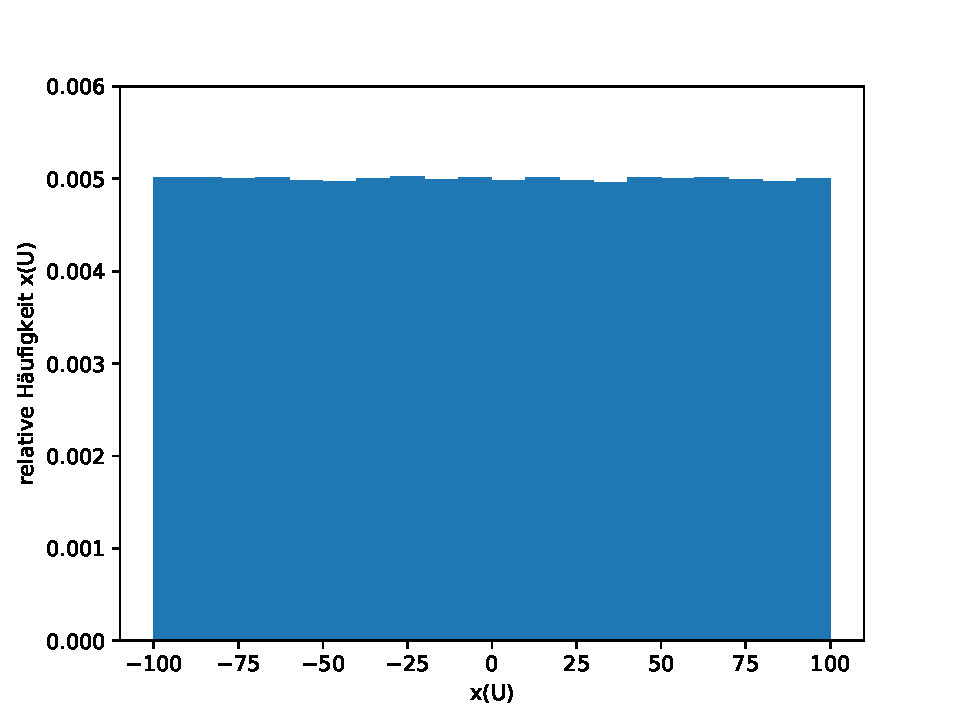
\includegraphics[scale=0.7]{Aufgabe05/Transformierte1.pdf}
  \caption{Transformierte Verteilung Aufgabenteil a).}
  \label{5.a}
\end{figure}


\subsection{b)}
Normierung:
\begin{align*}
  &\int_0^{\infty}N \exp{(-t/\tau)} \symup{d}t = \frac{-N}{\tau} \left[\exp{(-t/\tau)}\right]_0^{\infty} = \frac{N}{\tau} =1 \\
  => \; &N = \tau
\end{align*}
Transformation:
\begin{align*}
  U = \int_0^{t} \tau \cdot \exp{(-t'/\tau)} \symup{d}t' = -\exp{(-t/\tau)}+1 \\
\end{align*}
Inverse bilden:
\begin{align*}
  t(U) = - \tau \ln{(1-U)}
\end{align*}
Das zugehörige Histogramm ist in Abbildung \ref{5.b} zu sehen, dafür wurde für der Parameter als $\tau = 10$ angenommen und es
wurden 10000 Zufallswerte verwendet.
\begin{figure}[h]
  \centering
  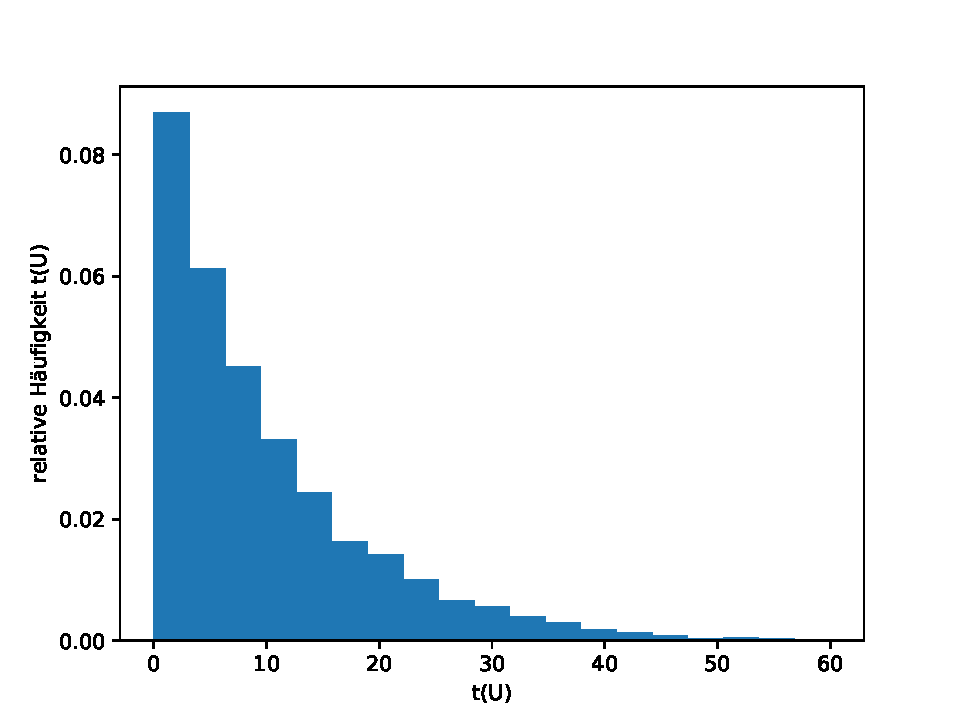
\includegraphics[scale=0.7]{Aufgabe05/Transformierte2.pdf}
  \caption{Transformierte Verteilung Aufgabenteil b).}
  \label{5.b}
\end{figure}

\subsection{c)}
Normierung:
\begin{align*}
  &\int_{x_{\symup{min}}}^{x_{\symup{max}}} N \cdot x^{-n} \symup{d}x = \frac{N}{1-n} \left[x^{1-n} \right]_{x_{\symup{min}}}^{x_{\symup{max}}}
  = \frac{N}{1-n}\left( x_{\symup{max}}^{1-n}-x_{\symup{min}}^{1-n} \right) = 1 \\
  => & N = \frac{1-n}{x_{\symup{max}}^{1-n}-x_{\symup{min}}^{1-n}}
\end{align*}
Transformation:
\begin{align*}
  U&=\int_{x_{\symup{min}}}^x \frac{1-n}{x_{\symup{max}}^{1-n}-x_{\symup{min}}^{1-n}} \cdot x'^{-n} \symup{d}x' \\
   &= \frac{1-n}{x_{\symup{max}}^{1-n}-x_{\symup{min}}^{1-n}}\left[\frac{1}{1-n} x'^{1-n} \right]_{x_{\symup{min}}}^x \\
   &= \frac{1}{x_{\symup{max}}^{1-n}-x_{\symup{min}}^{1-n}} \left( x^{1-n}-x_{\symup{min}}^{1-n} \right)
\end{align*}
Inverse bilden:
\begin{align*}
  x(U) = \left[ U \cdot \left( x_{\symup{max}}^{1-n}-x_{\symup{min}}^{1-n} \right) + x_{\symup{min}}^{1-n}  \right]   ^{\frac{1}{1-n}}
\end{align*}
Das zugehörige, normierte Histogramm ist in Abbildung \ref{5.c} zu sehen. Hierfür wurden folgende Werte angenommen:
\begin{align*}
  x_{\symup{min}} &= 1 \\
  x_{\symup{max}} &= 10 \\
  n&=2
\end{align*}
\begin{figure}[h]
  \centering
  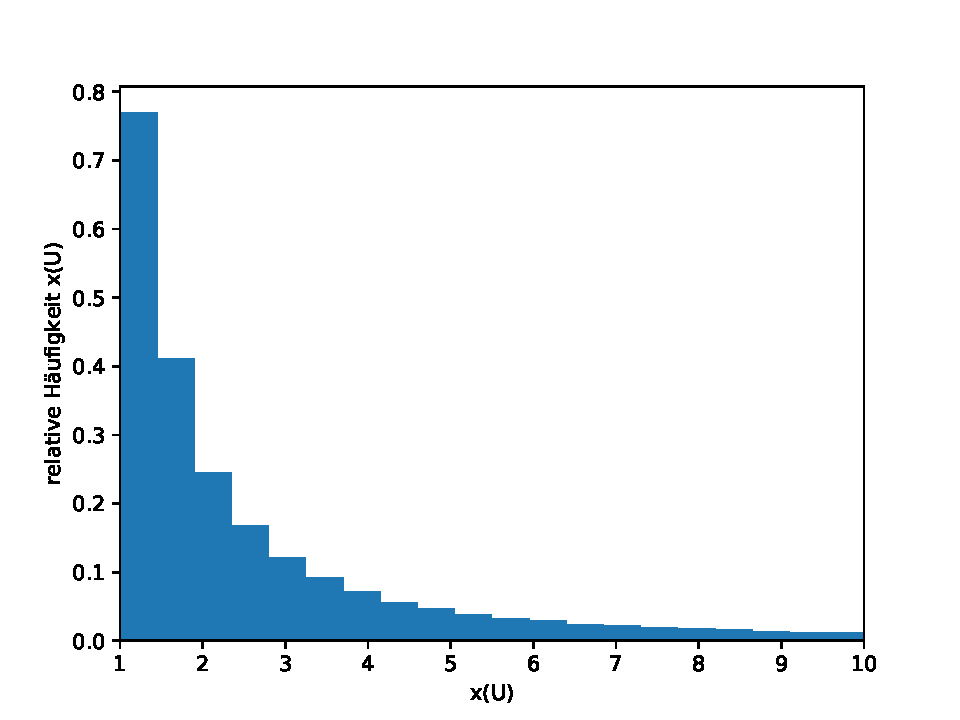
\includegraphics[scale=0.7]{Aufgabe05/Transformierte3.pdf}
  \caption{Transformierte Verteilung Aufgabenteil c).}
  \label{5.c}
\end{figure}

\subsection{d)}
Normierung ist hier nicht mehr notwendig, da die Funktion schon normiert ist.
Transformation:
\begin{align*}
  U &= \int_{-\infty}^{x} \frac{1}{\pi} \frac{1}{1+x'^2} \symup{d}x' \\
  &= \frac{1}{\pi} \left[ \arctan{(x')} \right]_{-\infty}^{x} \\
  &= \frac{1}{\pi} \left( \arctan{(x)}+ \frac{\pi}{2} \right)
\end{align*}
Inverse bilden:
\begin{align*}
  x(U) = \tan{\left( \pi \left(U-\frac{1}{2} \right) \right)}
\end{align*}
Das dazugehörige Histogramm ist in Abbildung \ref{5.d} zu sehen. Hierbei wurden erneut 1 Millionen Zufallszahlen verwendet.
\begin{figure}[h]
  \centering
  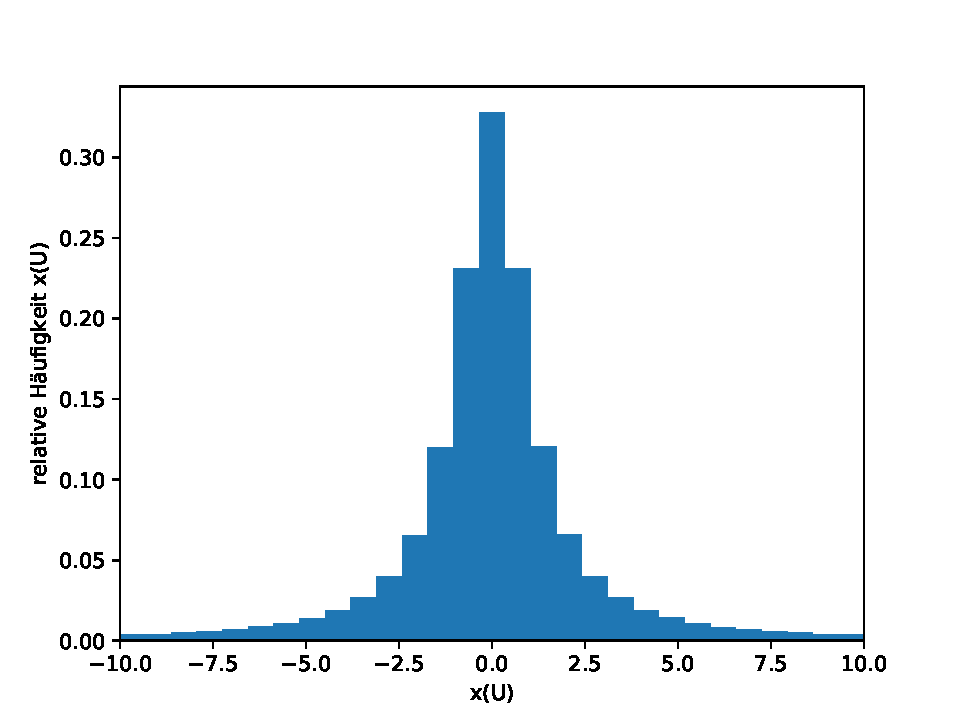
\includegraphics[scale=0.7]{Aufgabe05/Transformierte4.pdf}
  \caption{Transformierte Verteilung Aufgabenteil d).}
  \label{5.d}
\end{figure}
